\PassOptionsToPackage{usenames,dvipsnames}{xcolor}
\documentclass[tikz,border=2]{standalone}
\usepackage{amssymb}
\usepackage[scaled]{libertine}
%%\usepackage[scaled]{helvet}
\renewcommand{\familydefault}{\sfdefault} 
%%\usepackage{enumerate}
\usepackage{mathtools} % contains amsmath which comes with align
\usepackage{amsthm}
\usepackage{graphicx}
\usepackage{microtype} % some compression
\usepackage[skins]{tcolorbox}
\usepackage{enumitem} %\begin{itemize}[leftmargin=*,noitemsep,topsep=0pt]
%%%%%%%%%%
%% from https://www.gliffy.com/go/html5/launch?templateId=7033011
\definecolor{Red}{HTML}{C03316}
\definecolor{Orange}{HTML}{F7941C}
\definecolor{Green}{HTML}{A1B963}
\definecolor{Blue}{HTML}{3A5B8A}
\definecolor{LightBlue}{HTML}{4CC1EF}
%%
\def\labelitemi{\textcolor{gray}{\tiny{$\blacksquare$}}}

%% shift for arrow
\def\s{.14}
%%
%%%%%%%%%%%%%%%%%%%%%%%
\usetikzlibrary{shadows,arrows,shapes,positioning,calc,backgrounds,
fit,automata,decorations.markings,
decorations.pathreplacing,decorations.pathmorphing,spy}
%%%%%%%%%%%%%%%%%%%%%%%
\begin{document}
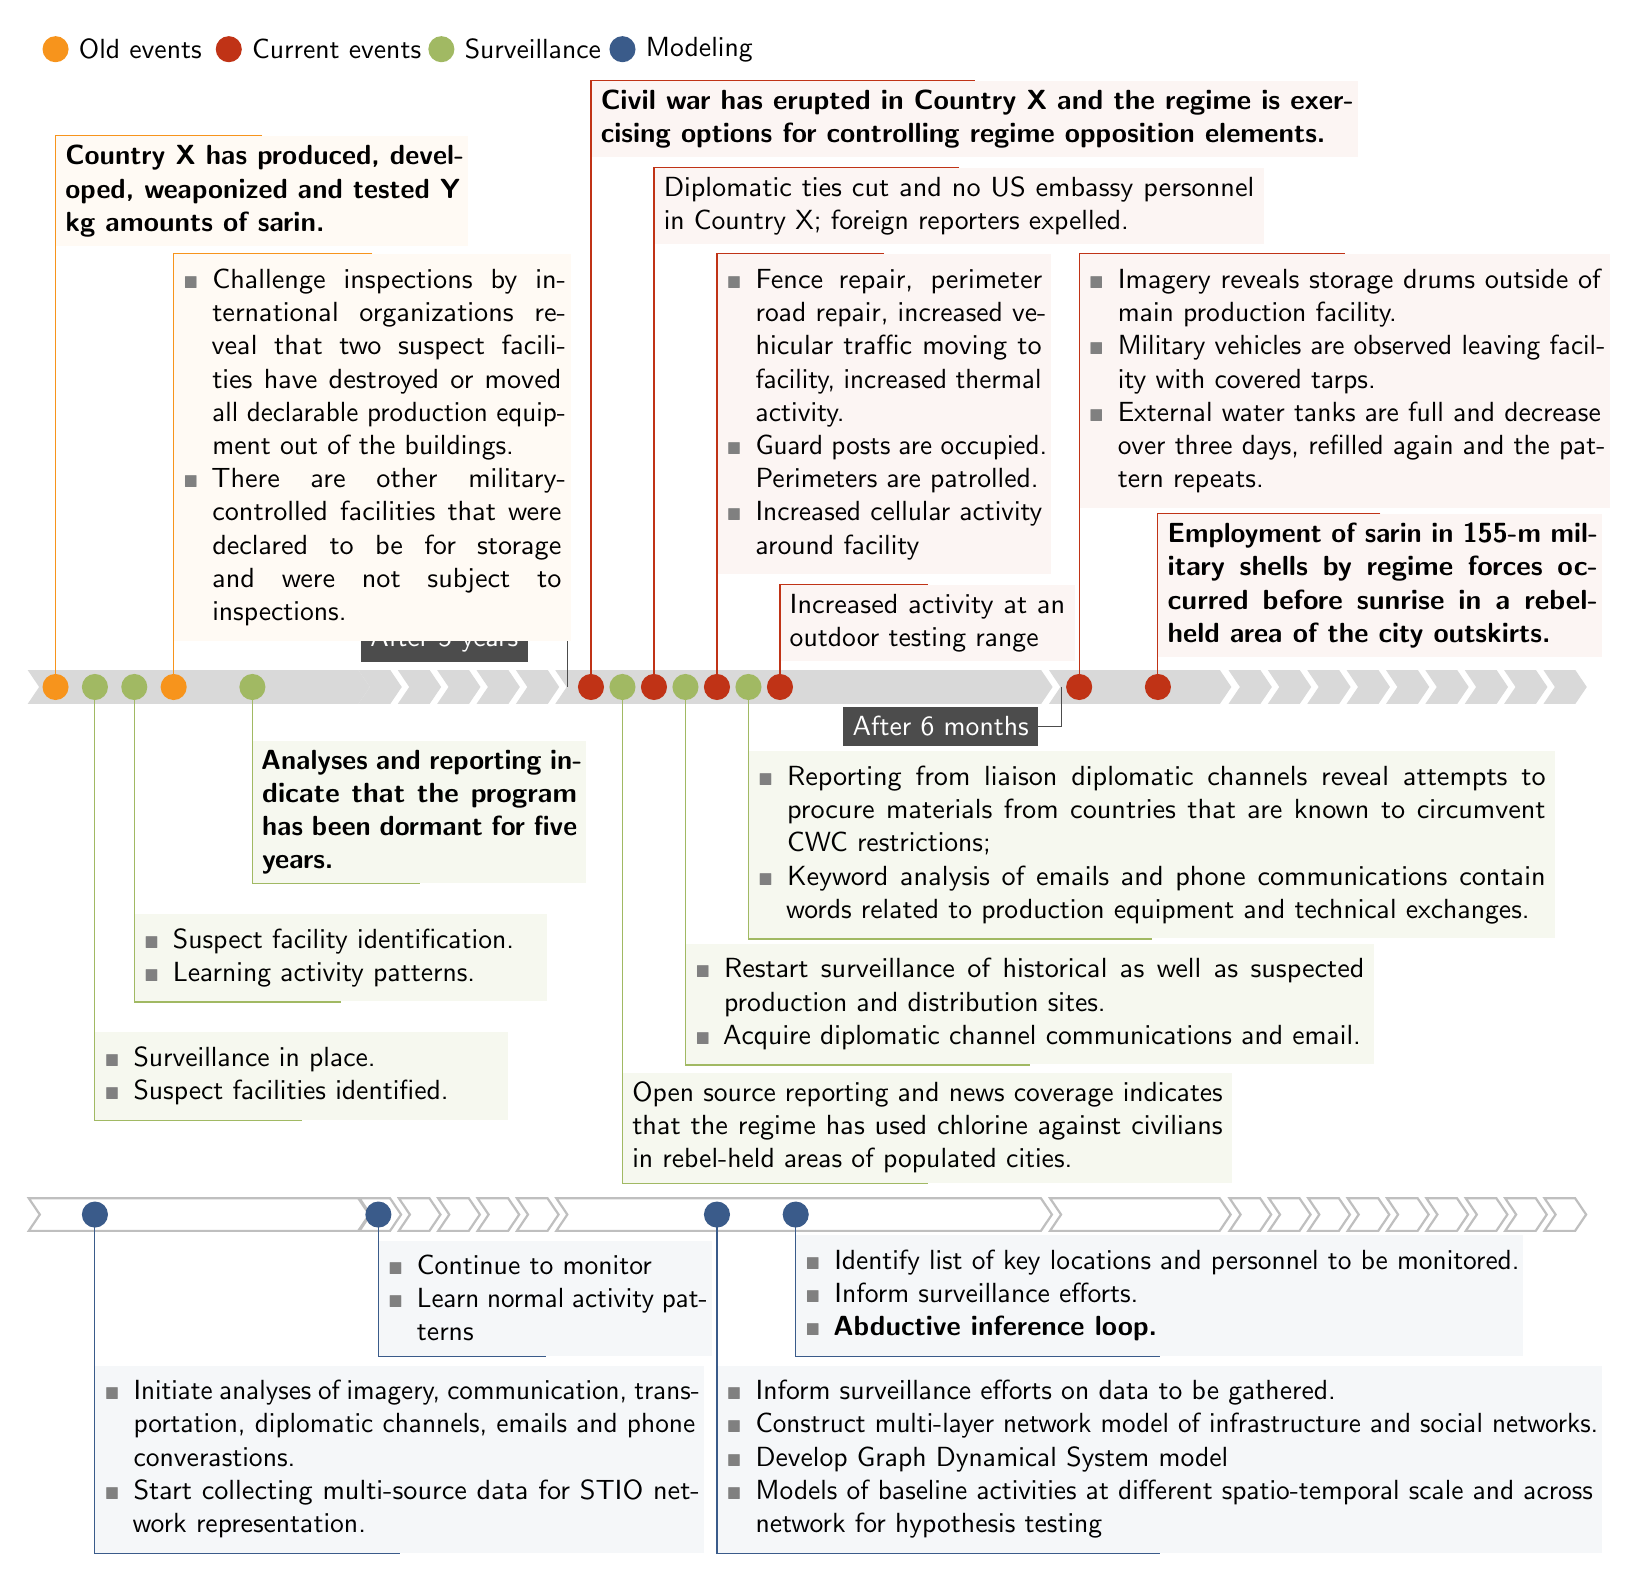
\begin{tikzpicture}
[scale=1,auto, transform shape,
%% blk/.style={rectangle,minimum height=5cm},
%% events/.style={blk,append after command={
%% \pgfextra{\draw[ultra thick,Red,fill,fill opacity=.1] 
%% ($(\tikzlastnode.north west)+(-\s,0)$) --
%% (\tikzlastnode.north east) -- 
%% ($(\tikzlastnode.east)+(\s,0)$) --
%% (\tikzlastnode.south east) --
%% ($(\tikzlastnode.south west)+(-\s,0)$) --
%% (\tikzlastnode.west) -- cycle;}
%% }},
blk/.style={rectangle},
timeline/.style={blk,anchor=west, minimum height=.4cm,append after command={
\pgfextra{\draw[black!15,fill]
($(\tikzlastnode.north west)+(-\s,0)$) --
(\tikzlastnode.north east) -- 
($(\tikzlastnode.east)+(\s,0)$) --
(\tikzlastnode.south east) --
($(\tikzlastnode.south west)+(-\s,0)$) --
(\tikzlastnode.west) -- cycle;}
}},
modelingTimeline/.style={blk,anchor=west, minimum height=.4cm,append after command={
\pgfextra{\draw[black!25,thick]
($(\tikzlastnode.north west)+(-\s,0)$) --
(\tikzlastnode.north east) -- 
($(\tikzlastnode.east)+(\s,0)$) --
(\tikzlastnode.south east) --
($(\tikzlastnode.south west)+(-\s,0)$) --
(\tikzlastnode.west) -- cycle;}
}},
pevent/.style={blk,fill=Orange!5,anchor=north west,append after command={
\pgfextra
\draw[thin,Orange] (\tikzlastnode.north) -|
(\tikzlastnode.north west|-{(0,0)}) node [circle,fill=Orange] {};
\endpgfextra
}},
event/.style={blk,fill=Red!5,anchor=north west,append after command={
\pgfextra
\draw[thin,Red] (\tikzlastnode.north) -|
(\tikzlastnode.north west|-{(0,0)}) node [circle,fill=Red] {};
\endpgfextra
}},
%%
response/.style={blk,fill=Green!10,anchor=south west,append after command={
\pgfextra
\draw[thin,Green] (\tikzlastnode.south) -|
(\tikzlastnode.south west|-{(0,0)}) node [circle,fill=Green] {};
\endpgfextra
}},
%%
modeling/.style={blk,fill=Blue!5,anchor=south west,append after command={
\pgfextra
\draw[thin,Blue] (\tikzlastnode.south) -|
(\tikzlastnode.south west|-{(0,0)}) node [circle,fill=Blue] {};
\endpgfextra
}},
pevents/.style={blk,ultra thick,draw=Red,fill=black!20},
presponse/.style={blk,draw=BurntOrange,fill=black!20},
pmodeling/.style={blk,draw=Purple,fill=black!20},
]
%% \newcommand{\block}[3]{\node[#1] {\parbox{#2}{#3}}}
%% past work
\node[pevent] (initEve) at (0,7) {\parbox{5cm}{
\bfseries Country X has produced, developed, weaponized and tested Y kg
amounts of sarin.
}};
%%
\node[response] (initSurv) at (.5,-5.5)
{\parbox{5cm}{
\begin{itemize}[leftmargin=*,noitemsep,topsep=0pt]
\item Surveillance in place.
\item Suspect facilities identified.
\end{itemize}
}};
%%
\node[response] (identify) at (1,-4)
{\parbox{5cm}{
\begin{itemize}[leftmargin=*,noitemsep,topsep=0pt]
\item Suspect facility identification.
\item Learning activity patterns.
\end{itemize}
}};
%%
\node[pevent] (inspection) at (1.5,5.5) {\parbox{4.8cm}{
\begin{itemize}[leftmargin=*,noitemsep,topsep=0pt]
\item Challenge inspections by international organizations reveal that 
two suspect facilities have destroyed or moved all declarable production
equipment out of the buildings. 
\item There are other military-controlled facilities that were declared to be
for storage and were not subject to inspections.
\end{itemize}
}};
%%
\node[response] (dormant) at (2.5,-2.5) {\parbox{4cm}{
\bfseries Analyses and reporting indicate that the program has been dormant for
five years.
}};
%%
\node[event] (civilWar) at (6.8,7.7) {\parbox{9.5cm}{
\bfseries Civil war has erupted in Country X and the regime is exercising
options for controlling regime opposition elements.
}};
%%
\node[response] (chlorine) at (7.2,-6.3) {\parbox{7.5cm}{
Open source reporting and news coverage indicates that the regime has
used chlorine against civilians in rebel-held areas of populated cities.
}};
%%
\node[event] (diplo) at (7.6,6.6) {\parbox{7.5cm}{
Diplomatic ties cut and no US embassy personnel in Country X; foreign
reporters expelled.
}};
%%
\node[response] (restartSurv) at (8,-4.8) {\parbox{8.5cm}{
\begin{itemize}[leftmargin=*,noitemsep,topsep=0pt]
\item Restart surveillance of historical as well as suspected production
and distribution sites.
\item Acquire diplomatic channel communications and email.
\end{itemize}
}};
%%
\node[event] (surveillanceActivities) at (8.4,5.5) {\parbox{4cm}{
\begin{itemize}[leftmargin=*,noitemsep,topsep=0pt]
\item Fence repair, perimeter road repair, increased vehicular
traffic moving to facility, increased thermal activity.
\item Guard posts are occupied. Perimeters are patrolled. 
\item Increased cellular activity around facility
\end{itemize}
}};
%%
\node[response] (emails) at (8.8,-3.2) {\parbox{10cm}{
\begin{itemize}[leftmargin=*,noitemsep,topsep=0pt]
\item Reporting from liaison diplomatic channels reveal attempts to procure
materials from countries that are known to circumvent CWC restrictions;
\item Keyword analysis of emails and phone communications contain words
related to production equipment and technical exchanges.
\end{itemize}
}};
%%
\node[event] (testing) at (9.2,1.3) {\parbox{3.5cm}{
Increased activity at an outdoor testing range
}};
%%
\node[event] (activitiesBeforeStrike) at (13,5.5) {\parbox{6.5cm}{
\begin{itemize}[leftmargin=*,noitemsep,topsep=0pt]
\item Imagery reveals storage drums outside of main production facility.
\item Military vehicles are observed leaving facility with covered tarps.
\item External water tanks are full and decrease over three days, refilled again and the pattern repeats.  
%% There is staining at the waste reservoir in back of production facility that is observed in imagery. Steam effluent is observed from air handling/scrubbers at rear roof of facility.
\end{itemize}
}};
%%
\node[event] (attack) at (14,2.2) {\parbox{5.4cm}{
\bfseries Employment of sarin in 155-m military shells by regime forces
occurred before sunrise in a rebel-held area of the city outskirts.
}};
%% timeline
\begin{pgfonlayer}{background}
\node[minimum width=4.03cm,timeline] at (-.2,0) {};
\foreach \x in {4,4.5,5,5.5,6}
\node[minimum width=0,timeline] at (\x,0) {};
\node[minimum width=6cm,timeline] at (6.5,0) {};
\node[minimum width=2cm,timeline] (sixmonth) at (12.77,0) {};
\draw[black!70] (6.5,0) |- (6,.6)
node[fill=black!70,draw,anchor=east,minimum height=.2cm,text=white] {After 5 years};
\draw[black!70] (sixmonth.west) |- (10,-0.5)
node[draw,anchor=west,fill=black!70,text=white,minimum height=.2cm] {After 6 months};
\foreach \x in {15.05,15.55,16.05,16.55,17.05,17.55,18.05,18.55,19.05}
\node[minimum width=0,timeline] at (\x,0) {};
\end{pgfonlayer}{background}
%% modeling
\begin{scope}[shift={(0,-6.7)}]
\node[minimum width=4.03cm,modelingTimeline] at (-.2,0) {};
\foreach \x in {4,4.5,5,5.5,6}
\node[minimum width=0,modelingTimeline] at (\x,0) {};
\node[minimum width=6cm,modelingTimeline] at (6.5,0) {};
\node[minimum width=2cm,modelingTimeline] (sixmonth) at (12.77,0) {};
\foreach \x in {15.05,15.55,16.05,16.55,17.05,17.55,18.05,18.55,19.05}
\node[minimum width=0,modelingTimeline] at (\x,0) {};
%%
\node[modeling] (initModel) at
(.5,-4.3) {\parbox{7.5cm}{
\begin{itemize}[leftmargin=*,noitemsep,topsep=0pt]
\item Initiate analyses of imagery, communication, transportation,
diplomatic channels, emails and phone converastions.
\item Start collecting multi-source data for STIO network representation.
\end{itemize}
}};
%%
\node[modeling] (monitor) at
(4.1,-1.8) {\parbox{4cm}{
\begin{itemize}[leftmargin=*,noitemsep,topsep=0pt]
\item Continue to monitor
\item Learn normal activity patterns
\end{itemize}
}};
%%
\node[modeling] (restart) at
(8.4,-4.3) {\parbox{11cm}{
\begin{itemize}[leftmargin=*,noitemsep,topsep=0pt]
\item Inform surveillance efforts on data to be gathered.
\item Construct multi-layer network model of infrastructure and social
networks.
\item Develop Graph Dynamical System model
\item Models of baseline activities at different spatio-temporal scale and
across network for hypothesis testing
\end{itemize}
}};
%%
\node[modeling] (restart) at
(9.4,-1.8) {\parbox{9cm}{
\begin{itemize}[leftmargin=*,noitemsep,topsep=0pt]
\item Identify list of key locations and personnel to be
monitored.
\item Inform surveillance efforts.
\item \bfseries Abductive inference loop.
\end{itemize}
}};
\end{scope}
%% legend
\begin{scope}[shift={(0,8.1)},name=legend]
\node[circle,fill=Orange,label=right:Old events] {};
\node[circle,fill=Red,label=right:Current events] at (2.2,0) {};
\node[circle,fill=Green,label=right:Surveillance] at (4.9,0) {};
\node[circle,fill=Blue,label=right:Modeling] at (7.2,0) {};
\end{scope}
\end{tikzpicture}
\end{document}
%%
